%------------------------------------------------------------------------------
% CV in Latex
% Author : Charles Rambo
% Based off of: https://github.com/sb2nov/resume and Jake's Resume on Overleaf
% Most recently updated version may be found at https://github.com/fizixmastr 
% License : MIT
%------------------------------------------------------------------------------

% \documentclass[A4,11pt]{article}
\documentclass[letterpaper,11pt]{article} %For use in US
\usepackage{iftex}
\ifXeTeX
  \usepackage{fontspec}
  \setmainfont{Times New Roman}
  \usepackage{xeCJK}
  \IfFontExistsTF{Songti SC}
    {\setCJKmainfont[BoldFont={Songti SC}, BoldFeatures={FakeBold=2}, ItalicFont={Kaiti SC}]{Songti SC}}
    {\IfFontExistsTF{Noto Serif CJK SC}
      {\setCJKmainfont{Noto Serif CJK SC}}
      {\IfFontExistsTF{Hiragino Sans GB}
        {\setCJKmainfont[BoldFont={Hiragino Sans GB W6}]{Hiragino Sans GB}}
        {\setCJKmainfont{WenQuanYi Zen Hei}}}}
\else\ifLuaTeX
  \usepackage{fontspec}
  \setmainfont{Latin Modern Roman}
  \usepackage{luatexja-fontspec}
  \setmainjfont{AR PL UMing CN}
\else
  \usepackage[utf8]{inputenc}
  \usepackage[T1]{fontenc}
\fi\fi
\usepackage{latexsym}
\usepackage[empty]{fullpage}
\usepackage{titlesec}
\usepackage{marvosym}
\usepackage[usenames,dvipsnames]{color}
\usepackage{verbatim}
\usepackage{enumitem}
\usepackage[hidelinks]{hyperref}
\usepackage[english]{babel}
\usepackage{tabularx}
\usepackage{graphicx}
\usepackage{tikz}
\usetikzlibrary{arrows.meta,calc,positioning}
\usepackage{xcolor}
% \input{glyphtounicode} % pdfTeX only, not needed for LuaLaTeX

\begin{comment}
I am by no means a professional when it comes to the CV's/resumes, I have
received various trainings on how to write a CV and resume from my high 
school, as well as the Austin College and University of Eastern Finland's
career counseling departments. As I intend to share my CV as a template, I 
feel that it is my responsibility to provide explanations of my work.
\end{comment}


%-----FONT OPTIONS-------------------------------------------------------------
\begin{comment}
The font of the document will impact not just how readable it is, but how it is
perceived. In the "The Craft of Scientific Writing" by Michael Alley, shares a
common fonts for publication as well as their use. I have chosen to use
Palatino for its legibility, some others are given below. There is far too much
about typography to discus here. Note: serif fonts have short projecting
strokes, sans-serif fonts are sans (without) these strokes.
\end{comment}


% serif - lmodern loaded at top before CJK for bold to work
% \usepackage{palatino} % deprecated, no bold support
% \usepackage{newpxtext} % modern Palatino with bold/italic support
% \usepackage{times} %This is the default as well
% \usepackage{charter} % bold not installed on this system

% sans-serif
% \usepackage{helvet}
% \usepackage[sfdefault]{noto-sans}
% \usepackage[default]{sourcesanspro}

%-----PAGE SETUP---------------------------------------------------------------

% Adjust margins
\addtolength{\oddsidemargin}{-1cm}
\addtolength{\evensidemargin}{-1cm}
\addtolength{\textwidth}{2cm}
\addtolength{\topmargin}{-1cm}
\addtolength{\textheight}{2cm}

% Margins for US Letter size
%\addtolength{\oddsidemargin}{-0.5in}
%\addtolength{\evensidemargin}{-0.5in}
%\addtolength{\textwidth}{1in}
%\addtolength{\topmargin}{-.5in}
%\addtolength{\textheight}{1.0in}

\urlstyle{same}

\raggedbottom
\raggedright
\setlength{\tabcolsep}{0cm}

% Sections formatting
\titleformat{\section}{
  \vspace{-4pt}\scshape\raggedright\large
}{}{0em}{}[\color{black}\titlerule \vspace{-5pt}]

% Ensure that .pdf is machine readable/ATS parsable
% \pdfgentounicode=1 % pdfTeX only, LuaLaTeX handles Unicode natively

%-----CUSTOM COMMANDS FOR FORMATTING SECTIONS----------------------------------
\newcommand{\CVItem}[1]{
  \item\small #1 \vspace{-2pt}
}

\newcommand{\CVSubheading}[4]{
  \vspace{-2pt}\item
    \begin{tabular*}{0.97\textwidth}[t]{l@{\extracolsep{\fill}}r}
      \textbf{#1} & #2 \\
      \small#3 & \small #4 \\
    \end{tabular*}\vspace{-7pt}
}

\newcommand{\CVSubSubheading}[2]{
    \item
    \begin{tabular*}{0.97\textwidth}{l@{\extracolsep{\fill}}r}
      \text{\small#1} & \text{\small #2} \\
    \end{tabular*}\vspace{-7pt}
}

\newcommand{\CVSubItem}[1]{\CVItem{#1}\vspace{-4pt}}
\newcommand{\ContactLink}[2]{\href{#1}{\underline{\strut #2}}}
\newcommand{\DOILink}[1]{\href{https://doi.org/#1}{doi:#1}}
\newcommand{\ArxivLink}[1]{\href{https://arxiv.org/abs/#1}{arXiv:#1}}
\newcommand{\ProjectLink}[2]{\href{#1}{#2}}

\renewcommand\labelitemii{$\vcenter{\hbox{\tiny$\bullet$}}$}

\newcommand{\CVSubHeadingListStart}{\begin{itemize}[leftmargin=0.5cm, label={}]}
% \newcommand{\resumeSubHeadingListStart}{\begin{itemize}[leftmargin=0.15in, label={}]} % Uncomment for US
\newcommand{\CVSubHeadingListEnd}{\end{itemize}}
\newcommand{\CVItemListStart}{\begin{itemize}}
\newcommand{\CVItemListEnd}{\end{itemize}\vspace{-5pt}}

\newcommand{\ResearchBlueBox}[6]{
  \node[
    draw=StoryBlue,
    fill=StoryLight,
    rounded corners=2pt,
    text width=#4cm,
    minimum height=1.55cm,
    align=left,
    inner sep=5pt,
    anchor=north west
  ] (#1) at (#2,#3) {
    \centering\color{StoryBlue}\textbf{#5}\par
    \vspace{2pt}
    \raggedright\scriptsize #6
  };
}
\newcommand{\ResearchGreenBox}[6]{
  \node[
    draw=StoryGreen,
    fill=StoryGreen!6,
    rounded corners=2pt,
    text width=#4cm,
    minimum height=0.82cm,
    align=left,
    inner sep=4pt,
    anchor=north west
  ] (#1) at (#2,#3) {
    \centering\color{StoryGreen}\textbf{#5}\par
    \vspace{1pt}
    \raggedright\tiny #6
  };
}
\newcommand{\ResearchFoundationBox}[6]{
  \node[
    draw=StoryBlue!55,
    fill=white,
    rounded corners=2pt,
    text width=4.25cm,
    minimum height=2.65cm,
    align=left,
    inner sep=5pt,
    anchor=north west
  ] (#1) at (#2,#3) {
    \centering\color{StoryBlue}\textbf{#4}\par
    \vspace{2pt}
    \raggedright\scriptsize #5\par
    \vspace{4pt}
    \raggedright\tiny #6
  };
}
\newcommand{\ResearchStoryDiagram}{
\begin{center}
\resizebox{\linewidth}{!}{%
\begin{tikzpicture}[font=\scriptsize]
  \definecolor{StoryBlue}{HTML}{0B4AA2}
  \definecolor{StoryLight}{HTML}{EAF1FB}
  \definecolor{StoryGreen}{HTML}{008C73}

  \node[anchor=west, color=StoryBlue, font=\scriptsize\bfseries] at (0,1.0)
    {Current direction: agents for LLM infrastructure on emerging AI chips};

  \ResearchBlueBox{agent}{0}{0}{3.65}{Native multi-agent architecture}
    {Programmable concurrent model\\Human-in-the-loop workflows\\Orchestration and workflow customization}
  \ResearchBlueBox{workflow}{5.0}{0}{4.05}{Agentic LLM infrastructure}
    {Layered operator-optimization skills\\Agent-native compiler stack\\Chip-aware performance optimization}
  \ResearchGreenBox{serving}{10.5}{0.05}{3.65}{LLM serving efficiency}
    {Efficient LLM serving\\on emerging AI chips.}
  \ResearchGreenBox{trajectory}{10.5}{-1.15}{3.65}{Development trajectories}
    {Real systems trajectories\\for stronger agents.}

  \draw[-{Latex[length=2mm]}, thick, StoryBlue]
    (agent.east) -- node[above, fill=white, inner sep=1pt, font=\tiny\bfseries] {apply to} (workflow.west);
  \draw[-{Latex[length=2mm]}, thick, StoryGreen]
    (workflow.north east) to[out=0,in=180]
    node[pos=0.53, above=3pt, fill=white, inner sep=1pt, font=\tiny\bfseries] {serve efficiently} (serving.west);
  \draw[-{Latex[length=2mm]}, thick, StoryGreen]
    (workflow.south east) to[out=0,in=180]
    node[pos=0.53, above=2pt, fill=white, inner sep=1pt, font=\tiny\bfseries] {capture data} (trajectory.west);
  \draw[-{Latex[length=2mm]}, thick, StoryGreen, rounded corners=5pt]
    (trajectory.east) -- (15.1,-1.6) |- (15.1,0.55) --
    node[above, fill=white, inner sep=1pt, font=\tiny\bfseries] {train stronger agents} (2.6,0.55) --
    (agent.north);

  \node[
    draw=StoryBlue!35,
    fill=StoryBlue!4,
    rounded corners=2pt,
    minimum width=15.1cm,
    minimum height=3.95cm,
    anchor=north west
  ] (foundation) at (-0.2,-3.0) {};
  \node[anchor=north, color=StoryBlue, font=\scriptsize\bfseries] at (7.35,-3.16)
    {Compiler-driven agile chip design foundations};
  \node[anchor=north, font=\tiny] at (7.35,-3.49)
    {Represent intent \(\rightarrow\) optimize implementations \(\rightarrow\) execute and observe};

  \draw[-{Latex[length=2mm]}, thick, StoryBlue]
    (2.2,-3.0) to[out=90,in=-90] node[fill=white, inner sep=1pt, font=\tiny\bfseries] {structured artifacts} (agent.south);
  \draw[-{Latex[length=2mm]}, thick, StoryBlue]
    (7.3,-3.0) to[out=90,in=-90] node[fill=white, inner sep=1pt, font=\tiny\bfseries] {optimization methods} (workflow.south);
  \draw[-{Latex[length=2mm]}, thick, StoryBlue]
    (12.3,-3.0) to[out=90,in=-70] node[fill=white, inner sep=1pt, font=\tiny\bfseries] {execution feedback} (workflow.south east);

  \ResearchFoundationBox{dsl}{0.1}{-4.02}{DSLs \& compiler stacks}
    {DSLs and multi-level IRs expose intent; compiler and synthesis passes lower it to executable designs.}
    {\ProjectLink{https://doi.org/10.1145/3508352.3549370}{Hector}, \ProjectLink{https://doi.org/10.1145/3626202.3637561}{Cement}\\
     \ProjectLink{https://doi.org/10.1109/ICCAD66269.2025.11240817}{APS}, \ProjectLink{https://uv-xiao.github.io/assets/pdf/aquas_iccad.pdf}{Aquas}}
  \ResearchFoundationBox{optimization}{5.1}{-4.02}{Architecture \& synthesis optimization}
    {Formal and e-graph search automate ISA, microarchitecture, and accelerator optimization.}
    {\ProjectLink{https://doi.org/10.1145/3779212.3790162}{ISAMORE}, \ProjectLink{https://doi.org/10.1109/ICCAD66269.2025.11240669}{Clay}, \ProjectLink{https://doi.org/10.1109/DAC63849.2025.11132875}{Cayman}\\
     \ProjectLink{https://arxiv.org/abs/2511.15323}{SkyEgg}, \ProjectLink{https://arxiv.org/abs/2604.17364}{EggMind}}
  \ResearchFoundationBox{execution}{10.1}{-4.02}{Execution \& co-design systems}
    {Inspectable artifacts, task graphs, and runtime feedback connect design intent to deployed systems.}
    {\ProjectLink{https://github.com/uv-xiao/IntelliC}{IntelliC}, \ProjectLink{https://github.com/hw-native-sys/simpler}{PTO Runtime}\\
     \ProjectLink{https://arxiv.org/abs/2604.17353}{Hive}, \ProjectLink{https://github.com/arch-of-shadow/spine}{Spine}}

  \draw[-{Latex[length=1.6mm]}, semithick, StoryBlue] (dsl.east) -- (optimization.west);
  \draw[-{Latex[length=1.6mm]}, semithick, StoryBlue] (optimization.east) -- (execution.west);
\end{tikzpicture}
}
\end{center}
}

%------------------------------------------------------------------------------
% CV STARTS HERE  %
%------------------------------------------------------------------------------
\begin{document}
%-----HEADING------------------------------------------------------------------
\begin{comment}
In Europe it is common to include a picture of ones self in the CV. Select
which heading appropriate for the document you are creating.
\end{comment}

% \begin{minipage}[c]{0.05\textwidth}
% \-\
% \end{minipage}
% \begin{minipage}[c]{0.2\textwidth}
% \begin{tikzpicture}
%     \clip (0,0) circle (1.75cm);
%     \node at (0,-.7) {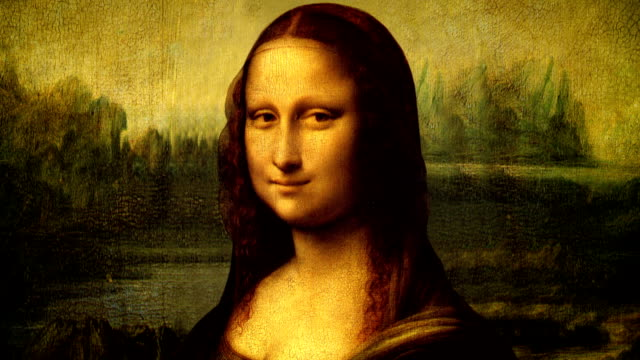
\includegraphics[width = 9cm]{portrait}}; 
%     % if necessary the picture may be moved by changing the at (coordinates)
%     % width defines the 'zoom' of the picture
% \end{tikzpicture}
% \hfill\vline\hfill
% \end{minipage}
% \begin{minipage}[c]{0.4\textwidth}
%     \textbf{\Huge {Youwei Xiao}} \\ \vspace{1pt} 
%     \small{Chinese Name: 肖有为} \\
%     % \scshape sets small capital letters, remove if desired
%     \small{+86 185 1920 4005} \\
%     \href{mailto:shallwe@pku.edu.cn}{\underline{shallwe@pku.edu.cn}}\\
%     % Be sure to use a professional *personal* email address
%     % \href{https://www.linkedin.com/in/charles-rambo/}{\underline{linkedin.com/in/charles-rambo}} \\
%     % you should adjust you linked in profile name to be professional and recognizable
%     % \href{https://github.com/fizixmastr}{\underline{github.com/fizixmastr}}
% \end{minipage}

% Without picture
\begin{center}
    \textbf{\Huge {Youwei Xiao}} \\ \vspace{1pt}
    \small{Chinese Name: {肖有为}} \\
    \small{+86 185 1920 4005} \\
    \small{\ContactLink{mailto:shallwe@pku.edu.cn}{shallwe@pku.edu.cn} \enspace\textbar\enspace
    \ContactLink{https://uv-xiao.github.io}{uv-xiao.github.io} \enspace\textbar\enspace
    \ContactLink{https://github.com/uv-xiao}{GitHub}}
\end{center}



\begin{comment}
This CV was written for specifically for positions I was applying for in
academia, and then modified to be a template.

A standard CV is about two pages long where as a resume in the US is one page.
sections can be added and removed here with this in mind. In my experience, 
education, and applicable work experience and skills are the most import things
to include on a resume. For a CV the Europass CV suggests the categories: Work
Experience, Education and Training, Language Skills, Digital Skills,
Communication and Interpersonal Skills, Conferences and Seminars, Creative Works
Driver's License, Hobbies and Interests, Honors and Awards, Management and
Leadership Skills, Networks and Memberships, Organizational Skills, Projects,
Publications, Recommendations, Social and Political Activities, Volunteering.

Your goal is to convey a who, what , when, where, why for every item you share. 
The who is obviously you, but I believe the rest should be done in that order.
For example below. An employer cares most about the degree held and typically 
less about the institution or where it is located (This is still good 
information though). Whatever order you choose be consistent throughout.
\end{comment}

%-----EDUCATION----------------------------------------------------------------
\section{Education}
  \CVSubHeadingListStart
%    \CVSubheading % Example
%      {Degree Achieved}{Years of Study}
%      {Institution of Study}{Where it is located}
    % \CVSubheading
    %   {{Master of Science $|$ \emph{\small{Photonics}}}}{Aug. 2019 -- May 2021}
    %   {University of Eastern Finland}{Joensuu, Finland}
    \CVSubheading
      {{Bachelor of Science degree in Computer Science}}{September 2018 - July 2022}
      {School of Electronics Engineering and Computer Science, Peking University}{Beijing, China}
    \CVSubheading
      {{Ph.D. Candidate in EDA}}{September 2022 - now}
      {School of Integrated Circuits, Peking University}{Beijing, China}
      \CVItemListStart
        \CVItem{Research: agents for LLM infrastructure on emerging AI chips, grounded in compiler-driven hardware-software co-design.}
      \CVItemListEnd
      % \CVItemListStart
      %   \CVItem{Relevant Coursework and Scores: Introduction to Computing(A)(Honor Track)(97/100), \ Practice of Programming in C\&C++(96/100), \ Introduction to Artificial Intelligence(88/100), \ Data Structure and Algorithm(A)(90/100), \ Introduction to Computer System(91/100),\ Practice of Data Structure and Algorithm(96/100), \ Algorithm Design and Analysis(86/100), \ Machine Learning(87/100), \ Computer Architectures(91/100), \ Lab on Computer Organization and Architecture(99/100), \ Principles of Compilers(91/100)}
      % \CVItemListEnd
    % \CVSubheading
    %   {Associate of Liberal Sciences}{Aug. 2015 -- May 2016}
    %   {North Lake College}{Irving, TX}
  \CVSubHeadingListEnd

\section{Work Experience}
  \CVSubHeadingListStart
    \CVSubheading
      {Large Language Model Algorithm Intern}{2026 -- Present}
      {ByteDance Seed}{Beijing, China}
      \CVItemListStart
        \CVItem{Contributed to native multi-agent coding systems, focusing on orchestration strategies and workflow customization with programmable concurrency and human-in-the-loop workflows.}
        \CVItem{Applied these approaches to LLM infrastructure by evolving an abstraction-layered operator-optimization skill system and an agent-native compiler stack for emerging AI chips.}
        \CVItem{Curated agent development data and trajectories from real systems tasks, turning infrastructure work into training signals for stronger coding and systems agents.}
      \CVItemListEnd
  \CVSubHeadingListEnd

\section{Research}

My current research centers on agents for LLM infrastructure on emerging AI chips. I contribute to native multi-agent coding systems by focusing on orchestration strategies and workflow customization through programmable concurrency and human-in-the-loop workflows. I apply these approaches by evolving an abstraction-layered operator-optimization skill system and an agent-native compiler stack, improving LLM serving efficiency while turning real development trajectories into training data for stronger coding and systems agents.

\ResearchStoryDiagram

\smallskip
\noindent \textbf{Compiler and runtime substrates.} Earlier systems work provides the surfaces that agents can operate on. \textit{IntelliC} (\ProjectLink{https://github.com/uv-xiao/IntelliC}{GitHub}) studies inspectable compiler representations for human-agent collaboration. \textit{PTO Runtime} (\ProjectLink{https://github.com/hw-native-sys/simpler}{GitHub}) executes compiled task graphs for serving on Ascend chips and LingQu SuperPods. \textit{Hive} (\ProjectLink{https://arxiv.org/abs/2604.17353}{preprint}) exposes multi-agent LLM workloads to inference infrastructure, while \textit{Spine} (\ProjectLink{https://github.com/arch-of-shadow/spine}{GitHub}) studies bounded agentic co-design across design intent, architecture, compiler, hardware, and execution evidence.

\smallskip
\noindent \textbf{Compiler-driven agile chip design.} My earlier research treats compilers as the organizing layer for architecture customization and hardware-software co-design. \textit{Hector} (\ProjectLink{https://doi.org/10.1145/3508352.3549370}{DOI}, \ProjectLink{https://github.com/pku-liang/Hector}{GitHub}) provides multi-level IRs for hardware synthesis; \textit{Cement} (\ProjectLink{https://doi.org/10.1145/3626202.3637561}{DOI}) couples the cycle-deterministic CmtHDL DSL with the CmtC timing-analysis and control-synthesis compiler; \textit{APS} (\ProjectLink{https://doi.org/10.1109/ICCAD66269.2025.11240817}{DOI}, \ProjectLink{https://github.com/pku-liang/APS}{GitHub}) builds an open-source MLIR stack from architecture DSLs to hardware synthesis and software compilation, and \textit{Aquas} (\ProjectLink{https://uv-xiao.github.io/assets/pdf/aquas_iccad.pdf}{ICCAD 2026}) extends it with domain-specific memory/synthesis directives and an e-graph retargetable compiler. \textit{Clay} (\ProjectLink{https://doi.org/10.1109/ICCAD66269.2025.11240669}{DOI}), \textit{Cayman} (\ProjectLink{https://doi.org/10.1109/DAC63849.2025.11132875}{DOI}), and \textit{SkyEgg} (\ProjectLink{https://arxiv.org/abs/2511.15323}{preprint}) automate microarchitecture and accelerator optimization, while \textit{ISAMORE} (\ProjectLink{https://doi.org/10.1145/3779212.3790162}{DOI}) and \textit{EggMind} (\ProjectLink{https://arxiv.org/abs/2604.17364}{preprint}) structure compiler search with formal and LLM-guided methods.

\smallskip
\noindent The resulting line of work uses earlier compiler and hardware systems as foundations for the next step: agents that help new chips serve LLM workloads, while the generated development data and trajectories feed back into stronger coding and systems models.


\section{Publications}

\CVItemListStart
\CVItem{\textbf{Youwei Xiao}, Chenyun Yin, Yitian Sun, and Yun Liang. 2026. Finding Reusable Instructions via E-Graph Anti-Unification. In Proceedings of the 31st ACM International Conference on Architectural Support for Programming Languages and Operating Systems (ASPLOS '26). \DOILink{10.1145/3779212.3790162}. \textbf{\textcolor{red}{[Best Paper Award, 5/1048]}}}
\CVItem{Yuyang Zou, \textbf{Youwei Xiao}, Yansong Xu, Chenyun Yin, Yuhao Luo, Yitian Sun, Ruifan Xu, Renze Chen, and Yun Liang. 2026. Aquas: Enhancing Domain Specialization through Holistic Hardware-Software Co-Optimization based on MLIR. In Proceedings of the 45th IEEE/ACM International Conference on Computer-Aided Design (ICCAD '26). \ProjectLink{https://uv-xiao.github.io/assets/pdf/aquas_iccad.pdf}{paper}.}
\CVItem{\textbf{Youwei Xiao}, Yuyang Zou, Yansong Xu, Yuhao Luo, Yitian Sun, Chenyun Yin, Ruifan Xu, Renze Chen, and Yun Liang. 2025. APS: Open-Source Hardware-Software Co-Design Framework for Agile Processor Specialization. In Proceedings of the 44th IEEE/ACM International Conference on Computer-Aided Design (ICCAD '25). \DOILink{10.1109/ICCAD66269.2025.11240817}. [Invited Paper]}
\CVItem{Weijie Peng*, \textbf{Youwei Xiao*}, Yuyang Zou, Zizhang Luo, and Yun Liang. 2025. Clay: High-level ASIP Framework for Flexible Microarchitecture-Aware Instruction Customization. In Proceedings of the 44th IEEE/ACM International Conference on Computer-Aided Design (ICCAD '25). \DOILink{10.1109/ICCAD66269.2025.11240669}. (*Equal contribution)}
\CVItem{\textbf{Youwei Xiao}, Fan Cui, Zizhang Luo, Weijie Peng, and Yun Liang. 2025. Cayman: Custom Accelerator Generation with Control Flow and Data Access Optimization. In Proceedings of the 62nd ACM/IEEE Design Automation Conference (DAC '25). \DOILink{10.1109/DAC63849.2025.11132875}.}
\CVItem{\textbf{Youwei Xiao}, Zizhang Luo, and Yun Liang. 2025. cmt2: Rule-Based Hardware Description in Rust with Temporal Semantics. In 5th Workshop on Languages, Tools, and Techniques for Accelerator Design (LATTE '25). \ProjectLink{https://capra.cs.cornell.edu/latte25/paper/1.pdf}{paper}.}
\CVItem{Fan Cui, \textbf{Youwei Xiao}, Kexing Zhou, and Yun Liang. 2025. An Empirical Comparison of LLM-based Hardware Design and High-level Synthesis. In Proceedings of the 2025 ACM/SIGDA International Symposium on Field Programmable Gate Arrays (FPGA '25). \DOILink{10.1145/3706628.3708861}.}
\CVItem{Fan Cui, Chenyang Yin, Kexing Zhou, \textbf{Youwei Xiao}, Guangyu Sun, Qiang Xu, Qipeng Guo, Yun Liang, Xingcheng Zhang, Demin Song, and Dahua Lin. 2024. OriGen: Enhancing RTL Code Generation with Code-to-Code Augmentation and Self-Reflection. In Proceedings of the 43rd IEEE/ACM International Conference on Computer-Aided Design (ICCAD '24). \DOILink{10.1145/3676536.3676830}.}
\CVItem{\textbf{Youwei Xiao}, Zizhang Luo, Kexing Zhou, and Yun Liang. 2024. Cement: Streamlining FPGA Hardware Design with Cycle-Deterministic eHDL and Synthesis. In Proceedings of the 2024 ACM/SIGDA International Symposium on Field Programmable Gate Arrays (FPGA '24). \DOILink{10.1145/3626202.3637561}.}
\CVItem{Ruifan Xu, \textbf{Youwei Xiao}, Jin Luo, and Yun Liang. 2022. HECTOR: A Multi-Level Intermediate Representation for Hardware Synthesis Methodologies. In Proceedings of the 41st IEEE/ACM International Conference on Computer-Aided Design (ICCAD '22). \DOILink{10.1145/3508352.3549370}.}
\CVItemListEnd

\section{Preprints}

\CVItemListStart
\CVItem{Chenyun Yin*, \textbf{Youwei Xiao*}, Yuze Luo, Yuyang Zou, and Yun Liang. LLM-Guided Strategy Synthesis for Scalable Equality Saturation. \ArxivLink{2604.17364}. (*Equal contribution)}
\CVItem{Zizhang Luo, Yuhao Luo, \textbf{Youwei Xiao}, Yansong Xu, Runlin Guo, and Yun Liang. Hive: A Multi-Agent Infrastructure for Algorithm- and Task-Level Scaling. \ArxivLink{2604.17353}.}
\CVItem{\textbf{Youwei Xiao}, Yuyang Zou, and Yun Liang. SkyEgg: Joint Implementation Selection and Scheduling for Hardware Synthesis using E-graphs. \ArxivLink{2511.15323}.}
\CVItem{\textbf{Youwei Xiao}, Zizhang Luo, Weijie Peng, Yuyang Zou, and Yun Liang. Cement2: Temporal Hardware Transactions for High-Level and Efficient FPGA Programming. \ArxivLink{2511.15073}.}
\CVItemListEnd



%-----HONORS AND AWARDS--------------------------------------------------------
\section{Honors and Awards}
  \CVSubHeadingListStart
    \CVSubheading
      {学术之芯}{2026}
      {Awarded to 8 students for academic excellence}{School of IC, Peking University}
    \CVSubheading
      {博士研究生校长奖学金}{2026-2027}
      {Awarded to 10 students in School of IC, Peking University}{Peking University}
    \CVSubheading
      {ASPLOS 2026 Best Paper Award}{March 2026}
      {Finding Reusable Instructions via E-Graph Anti-Unification}{5/1048 submissions}
    \CVSubheading
      {Second Place in EDAthon 2020}{August 2020}
      {Programming Competition on Electronic Design Automation}{IEEE CEDA Hong Kong Chapter}
    \CVSubheading
      {Shenzhen Stock Exchange Scholarship}{2019-2020}
      {Awarded to 17 students from EECS, Peking University}{}
    \CVSubheading
      {Merit Student}{2018-2019 \& 2019-2020}
      {Awarded to top 10\% students for comprehensive excellence}{}    
    \CVSubheading
      {Yang Fuqing \& Wang Yangyuan Academician Scholarship}{2018-2019}
      {Awarded to only 5 students at EECS, Peking University, for academic excellence}{}
    \CVSubheading
      {Second Prize in NOI 2017}{July 2017}
      {National Olympiad in Informatics}{China Computer Federation}
    \CVSubheading
      {Second Prize in APIO 2017}{May 2017}
      {Asia Pacific Informatics Olympiad (China District)}{China Computer Federation}
  \CVSubHeadingListEnd

%-----TUTORIALS----------------------------------------------------------------
\section{Tutorials}
  \CVSubHeadingListStart
    \CVSubheading
      {APS: An MLIR-Based Hardware-Software Co-design Framework}{January 2026}
      {ASP-DAC 2026}{Hong Kong, China}
    \CVSubheading
      {Agile Hardware Specialization: A toolbox for Agile Chip Front-end Design}{May 2025}
      {ISEDA 2025}{Hong Kong, China}
    \CVSubheading
      {Agile Hardware Specialization (AHS)}{March 2025}
      {ASPLOS 2025}{Rotterdam, Netherlands}
    \CVSubheading
      {Agile Hardware Specialization: A toolbox for Agile Chip Front-end Design}{March 2025}
      {DATE 2025}{Lyon, France}
    \CVSubheading
      {AHS: An EDA toolbox for Agile Chip Front-end Design}{January 2025}
      {ASP-DAC 2025}{Tokyo, Japan}
  \CVSubHeadingListEnd

%-----WORK EXPERIENCE----------------------------------------------------------
\begin{comment}
try to briefly explain what you did and why it is relevant to the position you
are seeking
\end{comment}

% \section{Work Experience}
%   \CVSubHeadingListStart
% %    \CVSubheading %Example
% %      {What you did}{When you worked there}
% %      {Who you worked for}{Where they are located}
% %      \CVItemListStart
% %        \CVItem{Why it is important to this employer}
% %      \CVItemListEnd
%     \CVSubheading
%       {Algorithm Intern}{June 2019 -- August 2019}
%       {Megvii(Beijing) Technology Co., Ltd}{Beijing, Mainland China}
%       \CVItemListStart
%         \CVItem{Intern of Video Team in Megvii Research}
%         \CVItem{Learned basic knowledge about single object tracking, mastered the basic usage of pyTorch}
%         \CVItem{Read papers SiamMask (CVPR2019) and ATOM(CVPR2019), retrained and tested the models}
%         \CVItem{Collected and sorted out several SOT datasets, contributing to the team's model improvement process}
%       \CVItemListEnd
%   \CVSubHeadingListEnd

%-----TEACHING EXPERIENCE------------------------------------------------------
% \section{Teaching Experience}
%   \CVSubHeadingListStart
%     \CVSubheading
%       {Teaching Assistant}{Fall 2020}
%       {Introduction to Computer Systems}{Peking University}
%     \CVSubheading
%       {Teaching Assistant}{Spring 2022 \& Fall 2022}
%       {High-level Chip Design}{Peking University}
%   \CVSubHeadingListEnd
  
%-----CONFERENCES AND PRESENTATIONS--------------------------------------------
% \begin{comment}
% Again the title should have already been enough, but if it is necessary to add
% descriptions maintain the consistency from prior sections
% \end{comment}

% \section{Conferences and Presentations}
%   \CVSubHeadingListStart
% %    \CVSubheading % Example
% %      {Work Presented}{When}
% %      {Occasion}{}
%     \CVSubheading
%       {Photometric Filter Fidelity and Use for Be Star Identification}{November 2017}
%       {Austin College Physics Research Seminar}{}
%     \CVSubheading
%       {Reflectometry for Volumetric Soil Moisture Measurement}{May 2017}
%       {Austin College Atmospheric Physics Fair}{}
%     \CVSubheading
%       {Design and Manufacturing of Products using 3D Printing}{April 2017}
%       {Austin College Student Scholarship Conference}{}
%   \CVSubHeadingListEnd

%-----COMMUNITY INVOLVEMENT----------------------------------------------------
% \section{Community Involvement}
%   \CVSubHeadingListStart
% %    \CVSubheading %Example
% %      {What you did}{When you worked there}
% %      {Who you worked for}{Where they are located}
%     \CVSubheading
%       {Austin College Community Tutors}{Fall 2017 -- Fall 2018}
%       {Free tutoring for local students in science and mathematics}{Sherman, TX}
%     \CVSubheading
%       {River Legacy Nature Center}{September 2015 -- August 2016}
%       {Provided assistance for various youth science education programs}{Arlington, TX}
%     \CVSubheading
%       {Back on My Feet Run Club}{April 2014 -- August 2015}
%       {Helping to reestablish homeless persons in the community}{Austin, TX}
%   \CVSubHeadingListEnd

%-----RESEARCH INTERESTS----------------------------------------------------------------

% \section{Research Interests}
% Currently, I'm working on the development of our own high-level synthesis flow, we plan to run through the flow, try more optimization passes and do experiments. I have a greatly strong willingness to build the next-generation open-source high-level synthesis tool, which is able to beat commercial HLS tools in broad application domains. I'm going to design multilevel IRs to support a variety of optimizations, try to integrate current frontier techniques for reference and explore brand new analysis and optimization methods
\end{document}
